\chapter{Interference, Diffraction, and the Doppler Effect}\index{interference}\index{diffraction}\index{Doppler effect}

An ambulance races past, and its siren drops in pitch the instant it passes you. Noise-cancelling
headphones make a jet engine go quiet by \emph{adding} more sound. A soap bubble shimmers with
colors that are not in the soap. You can hear someone talking around a corner but cannot see them.
And astronomers know the universe is expanding because light from distant galaxies is slightly
too red.

All of these come from what happens when waves meet each other or meet obstacles. In the
Introduction to Waves and Sound chapters, you studied one wave at a time. This chapter is about
waves combining (interference), waves bending around things (diffraction), and waves from moving
sources (the Doppler effect). Along the way, you will see the experiment that proved light is a wave.

\section{Superposition}\index{superposition}
When two waves overlap, the total disturbance at each point is simply the sum of the two. This is the
\newterm{principle of superposition}. Two water ripples that cross pass right through each other, and
where they overlap, their heights add.

\begin{figure}[H]
\centering
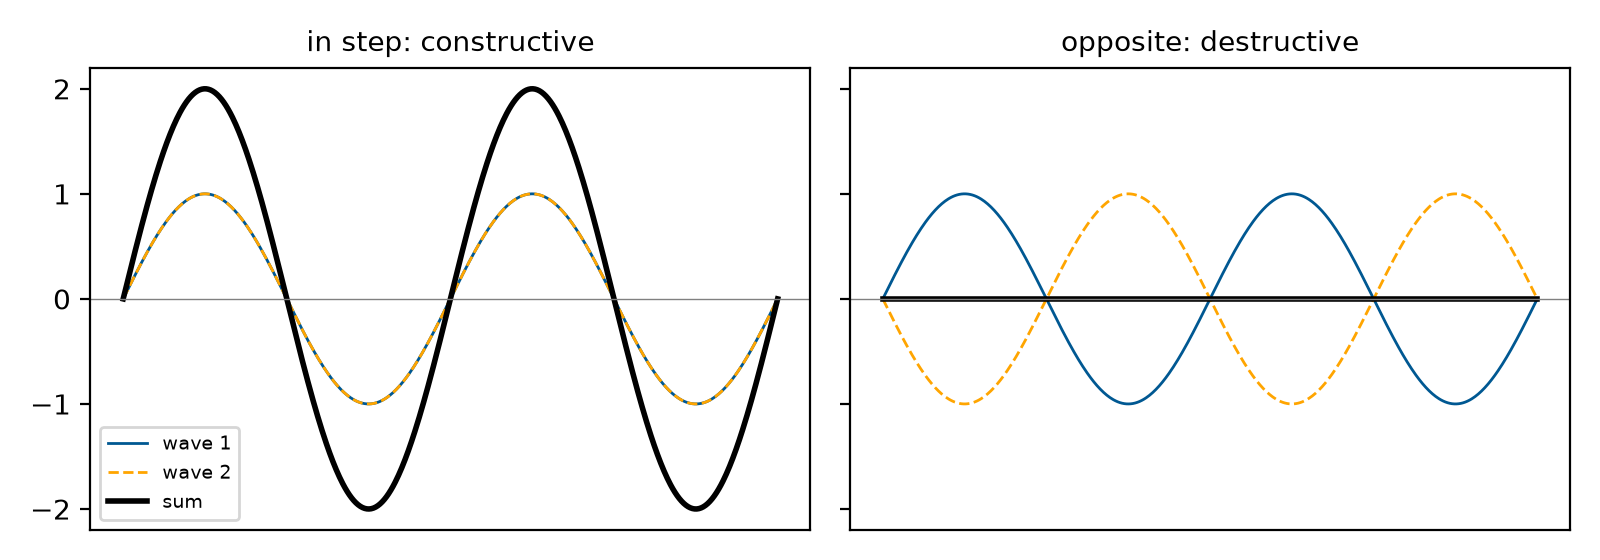
\includegraphics[width=0.9\textwidth]{superposition.png}
\caption{Left: two identical waves in step add to a wave twice as tall. Right: two waves exactly out of
step cancel completely.}
\label{fig:superposition}
\end{figure}

When crests meet crests, the waves reinforce each other: \newterm{constructive interference}. When crests
meet troughs, they cancel: \newterm{destructive interference}. Noise-cancelling headphones use a microphone
to record the noise around you, then play the same sound flipped upside down, crest for trough. The two
cancel inside your ear, and the drone of the engine fades.

\subsection{Beats}\index{beats}
What if two sounds have \emph{almost} the same frequency? They drift in and out of step. When they are in
step, the sound is loud; a moment later they are out of step, and it nearly vanishes. You hear a pulsing
``wah-wah-wah'' called \newterm{beats}.

The sum formulas from the Trigonometric Identities chapter show exactly what happens. Adding
$\sin(a + b)$ and $\sin(a - b)$ gives $\sin(a + b) + \sin(a - b) = 2\sin a\cos b$. With
$a = 2\pi\frac{f_1 + f_2}{2}t$ and $b = 2\pi\frac{f_2 - f_1}{2}t$, this becomes
$$\sin(2\pi f_2 t) + \sin(2\pi f_1 t) = 2\cos\left(2\pi\frac{f_2 - f_1}{2}t\right)\sin\left(2\pi\frac{f_1 + f_2}{2}t\right)$$
You hear a tone at the average frequency, whose loudness is controlled by the slowly changing cosine. The
loudness peaks twice per cycle of that cosine, so

\begin{mdframed}[style = important, frametitle = {Beat Frequency}]
$$f_{\text{beat}} = |f_1 - f_2|$$
\end{mdframed}

\begin{figure}[H]
\centering
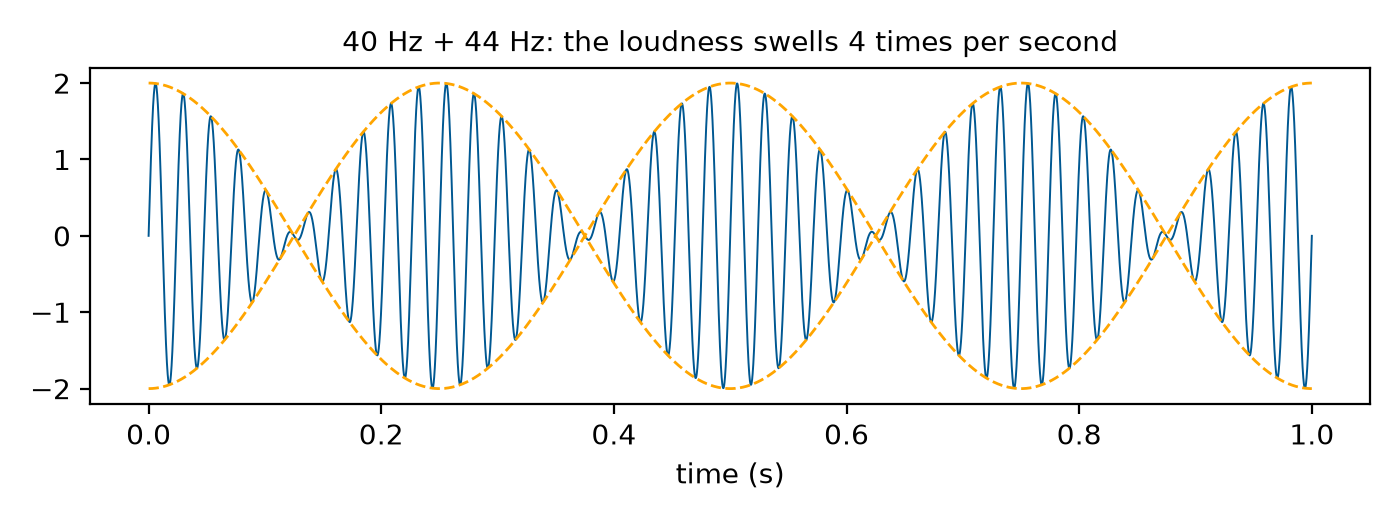
\includegraphics[width=0.85\textwidth]{beats.png}
\caption{Two tones 4 Hz apart produce 4 beats per second.}
\label{fig:beats}
\end{figure}

Musicians tune by ear this way. Play a guitar string along with a 440 Hz tuning note; if you hear 3 beats
per second, the string is 3 Hz off. Turn the peg until the beats slow down and disappear.

\begin{Exercise}[title={Adding Waves}, label=wv_add]
Two waves with amplitudes 3 cm and 2 cm pass through each other. What are the largest and smallest
possible amplitudes of the combined wave?
\end{Exercise}
\begin{Answer}[ref=wv_add]
In step, $3 + 2 = 5$ cm (constructive). Exactly out of step, $3 - 2 = 1$ cm (destructive). Unequal waves
cannot cancel completely.
\end{Answer}

\begin{Exercise}[title={Tuning a Guitar}, label=wv_beats]
A guitarist hears 3 beats per second when playing a string together with a 440 Hz tuning note. What are the
two possible frequencies of the string? The guitarist tightens the string slightly (raising its pitch), and
the beats speed up. Which frequency was it?
\end{Exercise}
\begin{Answer}[ref=wv_beats]
The string is at $440 \pm 3$: 437 Hz or 443 Hz. Tightening raises the pitch. If the beats speed up, the
string moved \emph{farther} from 440, so it was already above: 443 Hz. The guitarist should loosen it.
\end{Answer}

\section{Two Sources and the Double Slit}\index{double-slit experiment}
When waves from two sources overlap, whether they add or cancel at a point depends on how much farther one
wave traveled. If the \newterm{path difference} is a whole number of wavelengths, crests arrive with crests:
constructive. If it is a whole number plus a half, crests arrive with troughs: destructive.

\begin{mdframed}[style = important, frametitle = {Two-Source Interference}]
$$\text{constructive: } \Delta = m\lambda, \qquad \text{destructive: } \Delta = \left(m + \tfrac{1}{2}\right)\lambda, \qquad m = 0, 1, 2, \dots$$
where $\Delta$ is the path difference.
\end{mdframed}

You can hear this with two speakers playing the same tone: walk across the room, and the sound gets loud and
soft, loud and soft, as the path difference changes.

\subsection{Young's Experiment}
For centuries, scientists argued about whether light was a wave or a stream of tiny particles. In 1801, Thomas
Young settled it (for a hundred years, anyway) with a simple experiment. He passed light through two narrow
slits, very close together, onto a screen. Particles would make two bright stripes. Instead, he saw a row of
many bright and dark bands, called \newterm{fringes}: interference. Light is a wave.

\begin{figure}[H]
\centering
\begin{tikzpicture}[scale=1.25]
\fill[gray!40] (-0.08,0.62) rectangle (0.08,1.8);
\fill[gray!40] (-0.08,-0.38) rectangle (0.08,0.38);
\fill[gray!40] (-0.08,-1.8) rectangle (0.08,-0.62);
\draw[very thick] (6,-1.8) -- (6,2.6) node[above] {screen};
\coordinate (S1) at (0.08,0.5); \coordinate (S2) at (0.08,-0.5); \coordinate (P) at (6,2.2);
\draw[thick, sdkblue] (S1) -- (P);
\draw[thick, sdkblue] (S2) -- (P);
\draw[dashed] (0.08,0) -- (6,0);
\draw[dashed] (0.08,0) -- (P);
\draw (1.2,0) arc (0:20.1:1.12); \node at (1.45,0.22) {$\theta$};
\draw[thick, orange] (S1) -- (0.454,-0.332);
\draw[very thick, red] (S2) -- (0.454,-0.332);
\node[red, below right] at (0.25,-0.45) {$d\sin\theta$};
\draw[<->] (-0.35,0.5) -- (-0.35,-0.5) node[midway, left] {$d$};
\fill (P) circle (0.05) node[right] {$P$};
\draw[<->] (6.4,0) -- (6.4,2.2) node[midway, right] {$y$};
\draw[<->] (0.08,-2.05) -- (6,-2.05) node[midway, below] {$L$};
\end{tikzpicture}
\caption{Light from the lower slit travels farther to $P$ by the red segment, $d\sin\theta$. The real
screen is so far away compared with $d$ that the two rays are almost parallel.}
\label{fig:double-slit-geometry}
\end{figure}

Figure \ref{fig:double-slit-geometry} shows why the bands appear where they do. The slits are a distance $d$
apart. Light heading toward a point $P$ at angle $\theta$ from the lower slit travels farther than light from the
upper slit by $d\sin\theta$. So $P$ is bright when
$$d\sin\theta = m\lambda$$
In a real experiment, $\theta$ is tiny, so $\sin\theta \approx \tan\theta = \frac{y}{L}$, where $y$ is the distance
from the center of the screen and $L$ is the distance to the screen. The $m$th bright fringe is at
$y = \frac{m\lambda L}{d}$, and neighboring bright fringes are

\begin{mdframed}[style = important, frametitle = {Double-Slit Fringe Spacing}]
$$\Delta y = \frac{\lambda L}{d}$$
\end{mdframed}

\textbf{Example}: A red laser pointer ($\lambda = 650$ nm) shines through two slits 0.25 mm apart onto a wall 2.0 m
away. How far apart are the bright fringes?

\textbf{Solution}: $\Delta y = \frac{(650 \times 10^{-9})(2.0)}{0.25 \times 10^{-3}} = 5.2 \times 10^{-3}$ m, about 5 mm,
easy to see and measure. Turn the formula around, and a ruler can measure a wavelength of light,
a few ten-millionths of a meter.

The real pattern is shown below, computed in Python. The tall, narrow peaks are the two-slit fringes. They fade
toward the sides because each slit also spreads its light out on its own, which is the next topic.
\begin{minted}{python}
import numpy as np
import matplotlib.pyplot as plt

wavelength = 650e-9    # red laser, meters
d = 0.25e-3            # distance between the slits, meters
a = 0.04e-3            # width of each slit, meters
L = 2.0                # distance to the screen, meters

y = np.linspace(-0.04, 0.04, 4000)          # position on the screen, meters
theta = y / L                               # small-angle approximation

two_slit = np.cos(np.pi * d * theta / wavelength) ** 2
# np.sinc(x) means sin(pi x) / (pi x)
one_slit = np.sinc(a * theta / wavelength) ** 2
intensity = two_slit * one_slit

print(f"fringe spacing: {wavelength * L / d * 1000:.1f} mm")
print(f"central bright band: {2 * wavelength * L / a * 1000:.0f} mm wide")

plt.figure(figsize=(7, 3), dpi=200)
plt.plot(y * 1000, intensity)
plt.plot(y * 1000, one_slit, "--", color="orange")
plt.xlabel("position on screen (mm)")
plt.ylabel("brightness")
plt.tight_layout()
plt.savefig("double_slit.png")
\end{minted}
\begin{verbatim}
fringe spacing: 5.2 mm
central bright band: 65 mm wide
\end{verbatim}
\begin{figure}[H]
\centering
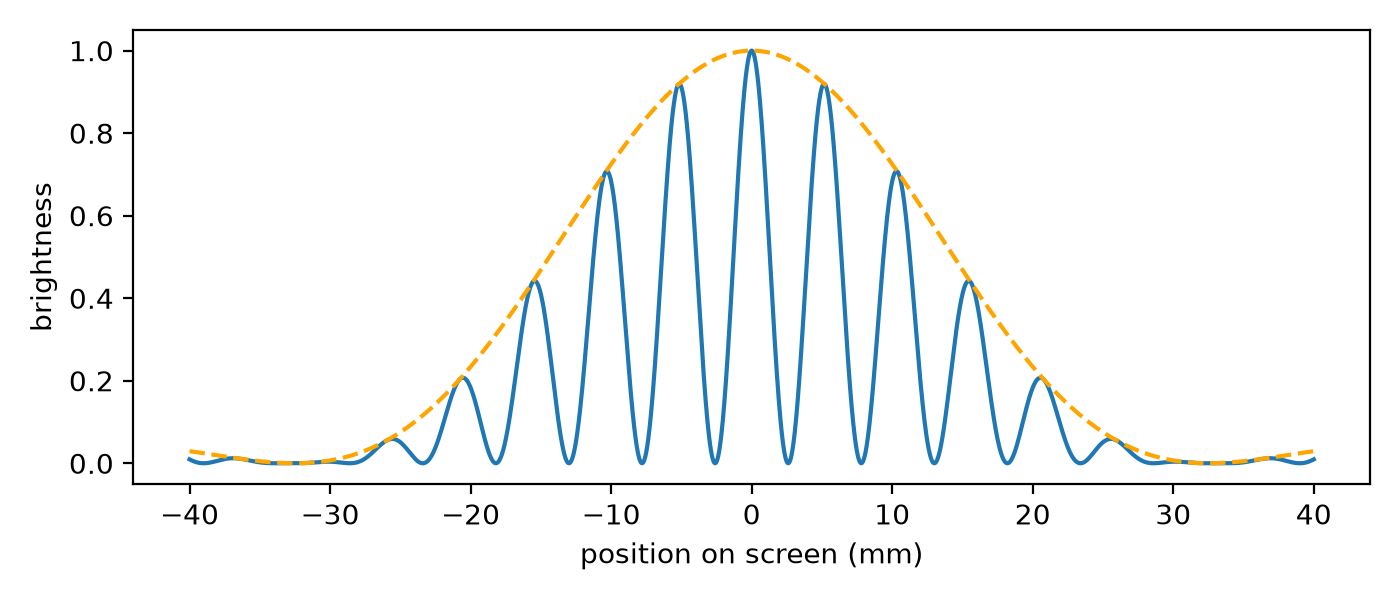
\includegraphics[width=0.85\textwidth]{double_slit.png}
\caption{The double-slit pattern. The dashed orange curve is the pattern from one slit alone.}
\label{fig:double-slit}
\end{figure}

A century after Young, the Photons chapter's discovery that light also comes in particles made this experiment
mysterious again. If you send photons through the slits \emph{one at a time}, each lands as a single dot, yet over
time the dots build up the same striped pattern. As the Paradoxes chapter put it, each photon somehow goes through
both slits. Physicists are still arguing about what that means.

\begin{Exercise}[title={Green Fringes}, label=wv_green]
A green laser ($\lambda = 532$ nm) shines through two slits 0.20 mm apart onto a screen 1.5 m away. Find the
fringe spacing.
\end{Exercise}
\begin{Answer}[ref=wv_green]
$\Delta y = \frac{(532 \times 10^{-9})(1.5)}{0.20 \times 10^{-3}} \approx 4.0 \times 10^{-3}$ m, about 4.0 mm.
\end{Answer}

\begin{Exercise}[title={Measuring Light with a Ruler}, label=wv_measure]
Light passes through two slits 0.30 mm apart onto a screen 2.0 m away. The bright fringes are 4.0 mm apart. What
is the wavelength? What color is it?
\end{Exercise}
\begin{Answer}[ref=wv_measure]
$\lambda = \frac{d\,\Delta y}{L} = \frac{(0.30 \times 10^{-3})(4.0 \times 10^{-3})}{2.0} = 6.0 \times 10^{-7}$ m $= 600$ nm,
which is orange light.
\end{Answer}

\section{Diffraction}\index{diffraction}
Waves spread out after passing through an opening or around an edge. This is \newterm{diffraction}, and how much a
wave spreads depends on the size of the opening compared with the wavelength. If the opening is much bigger than the
wavelength, the wave goes nearly straight through. If it is about the same size or smaller, the wave spreads widely.

That is why you can hear around a corner but not see around it. A voice at 500 Hz has a wavelength of
$\frac{343}{500} \approx 0.7$ m, about the size of a doorway, so it spreads around the corner. Visible light has a
wavelength of about 500 nm, more than a million times smaller than the doorway, so it travels in straight lines and
casts sharp shadows.

A single slit of width $a$ makes a wide central bright band with dark bands where $a\sin\theta = m\lambda$, for
$m = 1, 2, \dots$. That is the orange envelope in figure \ref{fig:double-slit}. The narrower the slit, the wider the
spread.

Diffraction also sets a limit on how sharply anything can see. Light passing through a telescope lens or a microscope
spreads by an angle of about $\frac{\lambda}{\text{width}}$, which blurs fine detail. Bigger telescopes and shorter
wavelengths see finer detail. That is why Blu-ray discs use a blue-violet laser instead of a DVD's red one: the shorter
wavelength focuses to a smaller spot, so the pits that store data can be packed more tightly.

\subsection{Diffraction Gratings}\index{diffraction grating}
A \newterm{diffraction grating} has thousands of evenly spaced slits. The bright fringes obey the same rule,
$d\sin\theta = m\lambda$, but with so many slits they become very sharp, and each color lands at a different angle.
The closely spaced tracks on a CD act as a grating, which is why it shines with rainbows. Astronomers attach gratings
to telescopes to split starlight into a spectrum and read which elements the star contains.

\begin{Exercise}[title={A Grating}, label=wv_grating]
A grating has 600 slits per millimeter. At what angle does the first-order ($m = 1$) red light ($\lambda = 650$ nm)
appear? What is the highest order of red light you can see?
\end{Exercise}
\begin{Answer}[ref=wv_grating]
$d = \frac{1}{600}$ mm $\approx 1.667 \times 10^{-6}$ m, so $\sin\theta = \frac{650 \times 10^{-9}}{1.667 \times 10^{-6}} \approx 0.39$
and $\theta \approx 23^\circ$. Since $\sin\theta$ cannot exceed 1, we need $m \leq \frac{d}{\lambda} \approx 2.56$, so the
highest order is $m = 2$.
\end{Answer}

\begin{Exercise}[title={Around the Corner}, label=wv_corner]
Explain why you can hear a friend talking in the hallway when you are in a classroom with the door open, even though
you cannot see them.
\end{Exercise}
\begin{Answer}[ref=wv_corner]
Sound waves from a voice have wavelengths around a meter, comparable to the width of the doorway, so they diffract,
spreading out around the corner into the room. Light has wavelengths about a million times smaller than the doorway,
so it barely diffracts and travels in straight lines.
\end{Answer}

\section{The Doppler Effect}\index{Doppler effect}
A source of waves sends out crests at a steady rate. If it is moving, each new crest starts from a slightly different
place. In front of the source, the crests bunch up; behind it, they spread out (figure \ref{fig:doppler}). Bunched-up
crests mean a shorter wavelength and a higher frequency. This is the \newterm{Doppler effect}, named after Christian
Doppler, who predicted it in 1842.

\begin{figure}[H]
\centering
\begin{tikzpicture}[scale=0.55]
\foreach \k in {1,...,5} {
  \draw[sdkblue, thick] ({-0.55*\k},0) circle (\k);
}
\fill[orange] (0,0) circle (0.15);
\draw[-latex, thick, orange] (0,0) -- (1.2,0);
\node[orange, above] at (0.6,0.1) {$v_s$};
\node at (6.4,0) {\small high pitch};
\node at (-9.4,0) {\small low pitch};
\end{tikzpicture}
\caption{Wavefronts from a source moving to the right. Each circle was emitted from where the source was at that time.
Crests crowd together ahead of the source and spread apart behind it.}
\label{fig:doppler}
\end{figure}

Here is the size of the effect. A source emits waves of frequency $f$ (period $T = \frac{1}{f}$), and the waves move
at speed $v$. If the source moves toward you at speed $v_s$, then in one period a crest travels $vT$ while the source
follows it by $v_sT$, so the next crest is only $(v - v_s)T$ behind. The wavelength you receive is $(v - v_s)T$, and the
frequency you hear is $\frac{v}{(v - v_s)T}$. For a source moving away, the minus sign becomes a plus.

\begin{mdframed}[style = important, frametitle = {The Doppler Effect for a Moving Source}]
$$f_{\text{heard}} = f\,\frac{v}{v - v_s} \text{ (approaching)}, \qquad f_{\text{heard}} = f\,\frac{v}{v + v_s} \text{ (receding)}$$
\end{mdframed}

\textbf{Example}: An ambulance siren sounds at 700 Hz, and the ambulance drives at 30 m/s. The speed of sound is
343 m/s. What do you hear as it approaches, and as it drives away?

\textbf{Solution}: Approaching: $700 \cdot \frac{343}{343 - 30} \approx 767$ Hz. Receding:
$700 \cdot \frac{343}{343 + 30} \approx 644$ Hz. As it passes, the pitch drops by more than 120 Hz, about three
musical half steps (the Sound chapter explained half steps).

The same idea works when you move instead of the source; then $f_{\text{heard}} = f\,\frac{v + v_o}{v}$ for an observer
moving toward the source at speed $v_o$. Police radar guns and weather radar bounce waves off moving cars or raindrops
and measure the frequency shift to find their speed. Doctors use Doppler ultrasound to watch blood flow through the heart.

\subsection{Sonic Booms}\index{sonic boom}
What happens as $v_s$ approaches the speed of sound $v$? The denominator $v - v_s$ shrinks to zero: the crests pile up on
top of each other in front of the source. A jet flying faster than sound outruns its own sound waves, which merge into a
cone-shaped shock wave trailing behind it. When the cone sweeps over you, you hear a single loud \newterm{sonic boom}.
A whip's crack is a tiny sonic boom: the tip moves faster than sound.

\subsection{Redshift}\index{redshift}
Light shows a Doppler effect too. For a source moving away at a speed $v$ much less than the speed of light $c$, the
wavelength stretches by
$$\frac{\Delta\lambda}{\lambda} \approx \frac{v}{c}$$
so the light looks a little redder: a \newterm{redshift}. In the 1920s, Edwin Hubble found that nearly every distant galaxy
is redshifted, and the farther away it is, the faster it is receding. The universe is expanding.

\textbf{Example}: Hydrogen gives off red light at 656.3 nm. In a distant galaxy, that line is observed at 662.9 nm. How
fast is the galaxy moving away?

\textbf{Solution}: $v \approx c\,\frac{\Delta\lambda}{\lambda} = (3.00 \times 10^5 \text{ km/s})\frac{662.9 - 656.3}{656.3} \approx 3{,}000$ km/s.

\begin{Exercise}[title={A Passing Train}, label=wv_train]
A train horn sounds at 400 Hz, and the train moves at 25 m/s. The speed of sound is 343 m/s. What frequencies do you
hear as the train approaches and as it moves away?
\end{Exercise}
\begin{Answer}[ref=wv_train]
Approaching: $400 \cdot \frac{343}{318} \approx 431$ Hz. Receding: $400 \cdot \frac{343}{368} \approx 373$ Hz.
\end{Answer}

\begin{Exercise}[title={A Faster Galaxy}, label=wv_galaxy]
In another galaxy, the 656.3 nm hydrogen line is observed at 669.4 nm. About how fast is the galaxy receding?
\end{Exercise}
\begin{Answer}[ref=wv_galaxy]
$v \approx (3.00 \times 10^5)\frac{669.4 - 656.3}{656.3} \approx 6{,}000$ km/s, about twice as fast as the galaxy in the
example. By Hubble's discovery, it is also about twice as far away.
\end{Answer}
